\chapter{Implementation}
This chapter highlights the implementational aspects of the system. Introducing the technologies used to build the components. Each section title is referring to its respective GitHub repository of the \texttt{ARTIS-project}\footnote{\href{https://github.com/artis-project/}{https://github.com/artis-project/}} GitHub organization.

\section{artis-rockpi-logger}

\begin{wrapfigure}[15]{o}{0.5\textwidth}
    \centering
    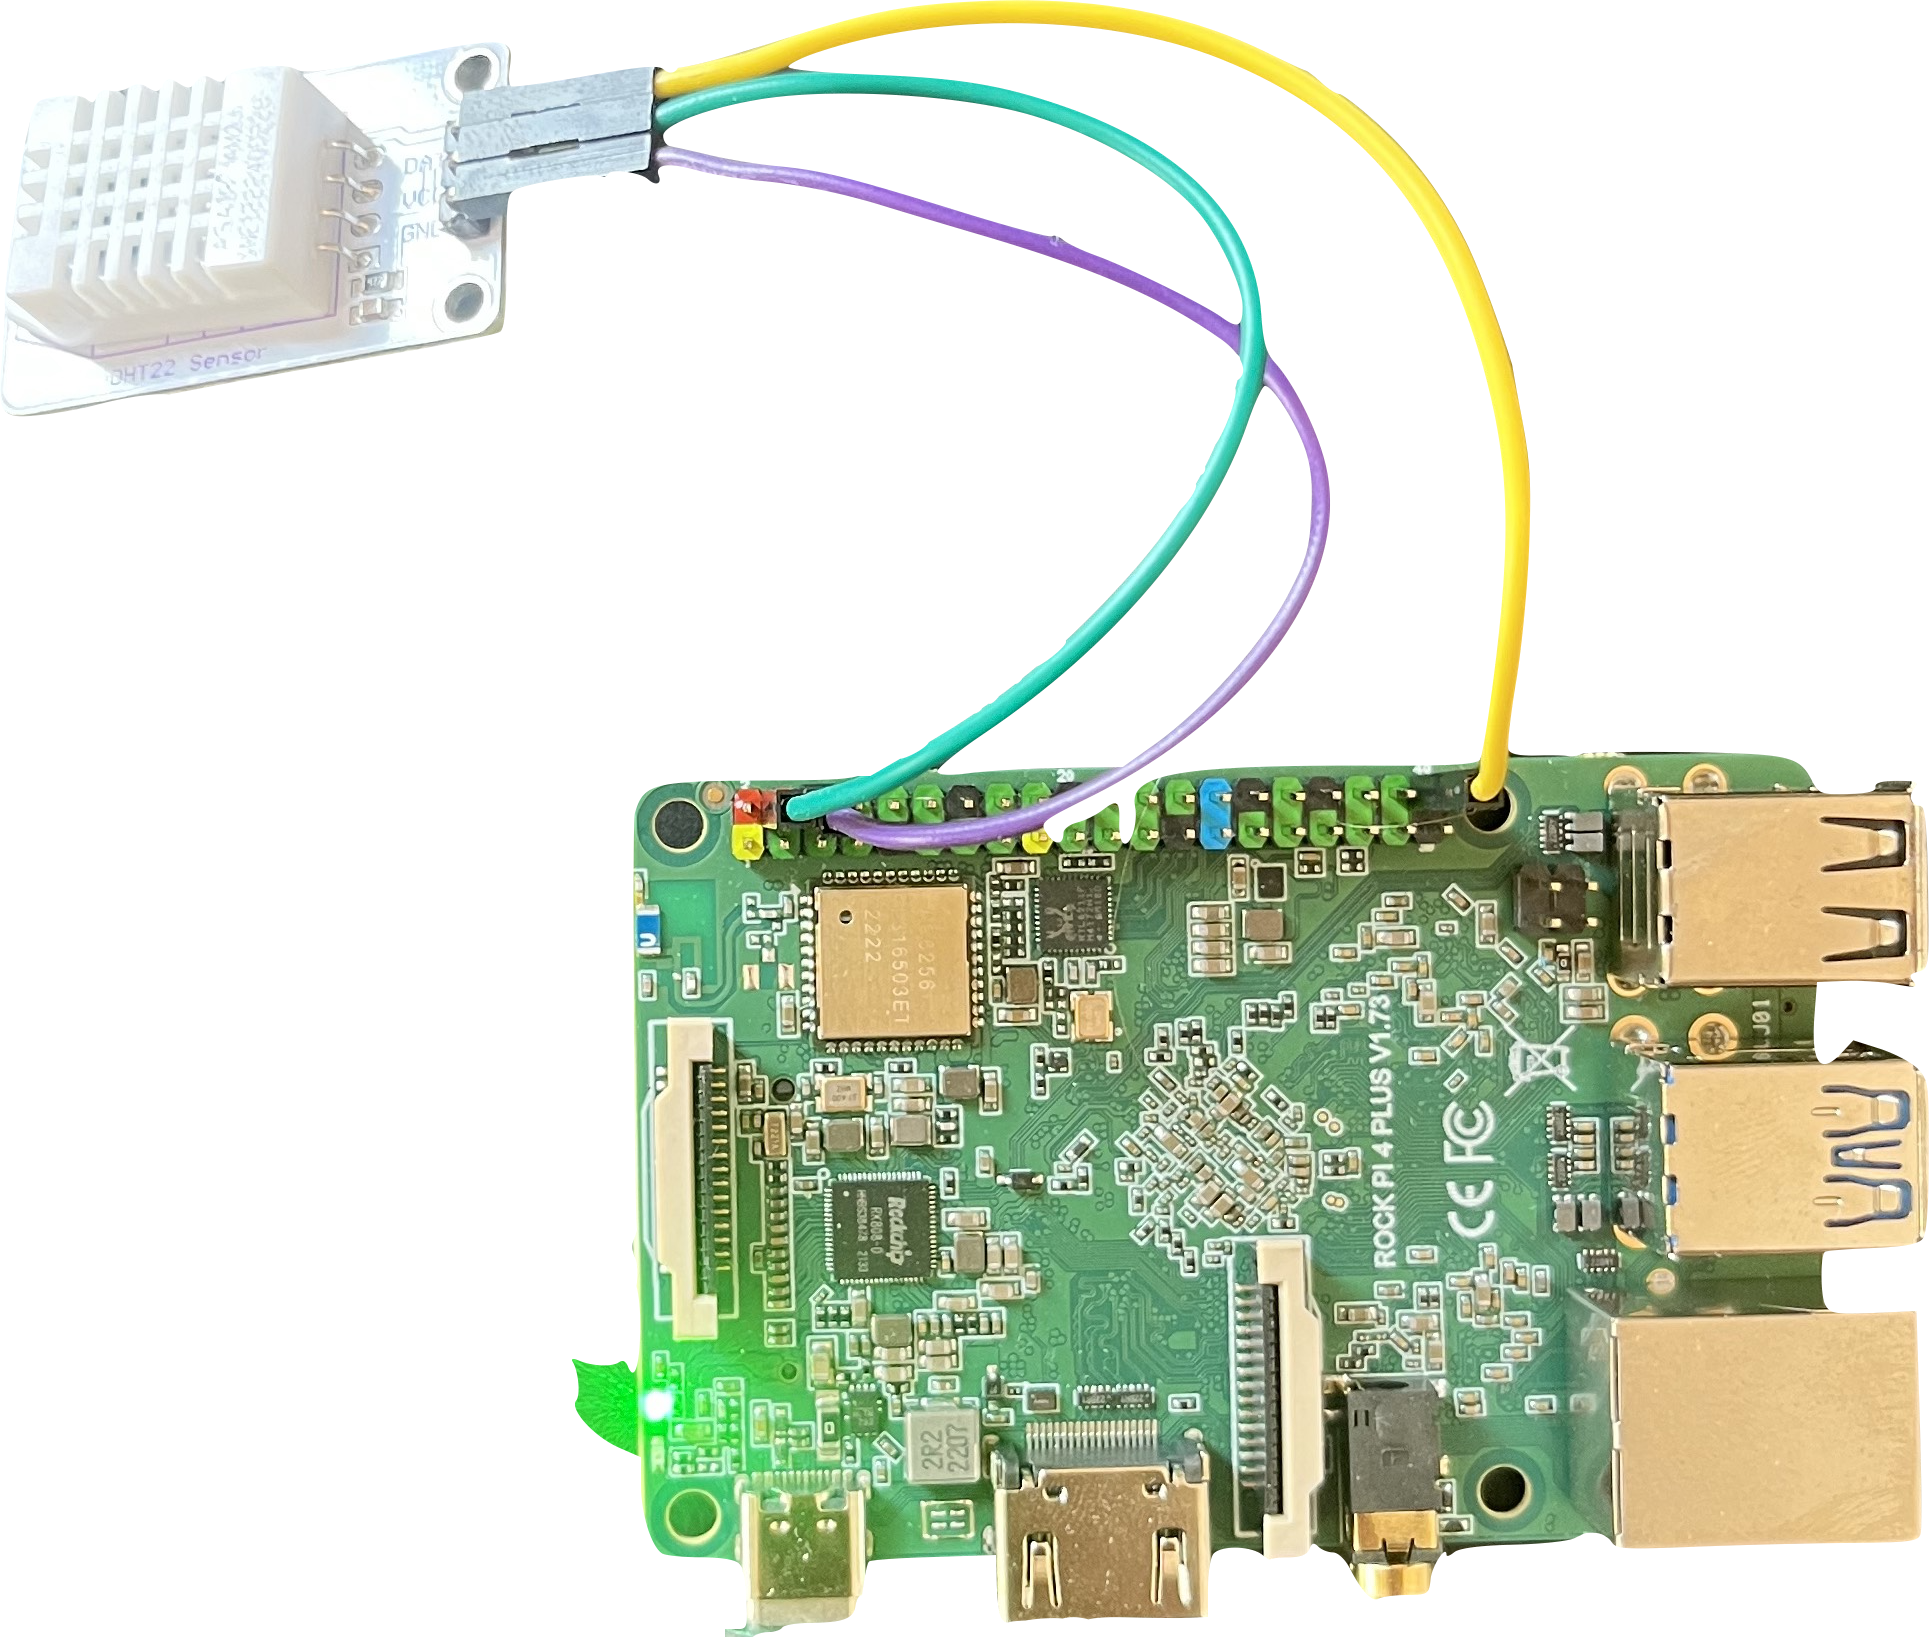
\includegraphics[width=0.49\textwidth]{resources/rock-pi.png}
    \caption{Rock Pi with a DHT-22 sensor} 
    \label{fig:rock-pi}
\end{wrapfigure}

For this project, we used a Rock Pi \footnote{\href{https://rockpi.org/rockpi4}{https://rockpi.org/rockpi4}} with a DHT-22\footnote{\href{https://www.adafruit.com/product/385}{https://www.adafruit.com/product/385}} sensor attached. (Figure \ref{fig:rock-pi})

The decision for this device and sensor is based on simplicity and flexibility as well as on low acquisition costs. The Rock Pi is compatible with Linux operating systems which makes it very simple to write scripts using high-level programming languages like Python. It also has \gls{gpio} support to easily connect the DHT-22 sensor. The sensor is capable of recording temperature and humidity data from the environment.

\begin{figure}
    \centering
    \begin{forest}
      for tree={
        font=\ttfamily,
        grow'=0,
        child anchor=west,
        parent anchor=south,
        anchor=west,
        calign=first,
        edge path={
          \noexpand\path [draw, \forestoption{edge}]
          (!u.south west) +(7.5pt,0) |- node[fill,inner sep=1.25pt] {} (.child anchor)\forestoption{edge label};
        },
        before typesetting nodes={
          if n=1
            {insert before={[,phantom]}}
            {}
        },
        fit=band,
        before computing xy={l=15pt},
      }
    [artis-rockpi-logger
      [/Rockfruit\_Python\_DHT
      ]
      [artis\_api.py
      ]
      [authenticator.py
      ]
      [logging\_script.py
      ]
      [violation\_script.py
      ]
    ]
    \end{forest}
    \caption{Filetree of the artis-rockpi-logger repository}
    \label{fig:artis-logger-filetree}
\end{figure}

\subsection{Sensor Interface}
To read data from the DHT-22 sensor we used an existing library called Rockfruit\_Python\_DHT\footnote{\href{https://github.com/Tim-J-Parbs/Rockfruit_Python_DHT}{https://github.com/Tim-J-Parbs/Rockfruit\_Python\_DHT}} that we adapted slightly to work with our board. The library provides a function with the signature \texttt{read\_retry(sensor, pin, retries=15, delay\_seconds=2)}. This method reads data from the DHT sensor of the specified type (in our case 22) on the specified \gls{gpio} pin and returns a tuple of humidity (as a floating point value in percent) and temperature (as a floating point value in Celsius). The function will attempt to read multiple times (up to the specified retries) until a reading can be registered. If no reading can be registered after the amount of retries the function will return \texttt{(None, None)}. The default delay between retries is two seconds but can be overridden.

\lstinputlisting[
    language=Python,
    caption=Temperature and humidity logging loop in \texttt{logging\_script.py},
    label=lst:loggingscript
]{codesnippets/logging_script.py}    

In Listing \ref{lst:loggingscript} you can see the that the script is executing the \texttt{read\_retry} function in an endless loop and whenever the reading has been successful it stores the data along with a timestamp of the reading in seconds and in a readable format in a local database.

The logger contains a second important script which is run simultaneously. The \texttt{violation\_script.py} is executed with the predefined temperature and humidity thresholds and the corresponding artwork id.

\lstinputlisting[
    language=bash,
    caption=Executing the \texttt{violation\_script.py},
    label=lst:violationscript,
    xleftmargin=2cm,
    xrightmargin=2cm
]{codesnippets/violation_script.py}

This script contains another while loop that continuously checks for new entries in the database and evaluates whether the threshold has been exceeded. If there has been either a temperature or humidity violation the script calls the corresponding method to call the \texttt{ARTIS} server \gls{api}. These methods are defined in the \texttt{artis\_api.py} file.

To authenticate to the \gls{api}, the logger follows the same authentication flow illustrated in Figure \ref{fig:auth_flow}. The methods used to send the authentication requests and sign the challenge message are defined in the \texttt{authenticator.py} file.

\section{artis-smartcontract}

The \gls{sc} was written in Ethereum's native programming language Solidity \cite{solidity}. The contract was developed using hardhat \cite{hardhat}, a development environment for Ethereum. Hardhat makes it easy to develop, compile, test, and deploy smart contracts. The \gls{sc} has been deployed to the Ethereum testnet Sepolia \cite{sepolia} during development, but is intended to be deployed on the mainnet in production. The Ethereum blockchain was selected due to prior experience of the research group and the author.

When the \gls{sc} is first deployed the smartcontract admin is set to the deploying address. This address will be the only point of access to any \gls{sc} function. It is also the account used by the server to interact with the \gls{sc} and sign transactions.

\lstinputlisting[
    language=Solidity,
    caption=\gls{sc} constructor function,
    label=lst:scconstructor,
    firstline=53,
    lastline=55
]{codesnippets/smartcontract.sol}

As seen in Listing \ref{lst:scconstructor} the \gls{sc} extends the ERC721 \cite{erc721} contract which provides the \gls{nft} interface.

\subsection{Data Structures and Events}
To understand the rest of the contract we will explain the data structures used in more detail.

\subsubsection{Structs}
To satisfy the artwork tracking use case three additional structs have been defined as seen in Listing \ref{lst:scstructs}. The \texttt{ArtworkData} struct contains all information about a specific artwork. This includes the addresses of each actor as well as the violation timestamp and the status of the artwork. The status field in turn contains to fields as defined in the \texttt{Status} struct. They are used to support the multi-approval process when it comes to changing the status of an artwork. To match the physical artwork with the \gls{nft} we also included an objectID field. The \texttt{ArtworkData} struct can be extended with more data fields if needed.

The \texttt{StatusApprovals} struct is used to store which of the actors has already approved a status change. The logic behind this multi-approval process will be explained in detail later.

\lstinputlisting[
    language=Solidity,
    caption=\gls{sc} structs,
    label=lst:scstructs,
    firstline=1,
    lastline=20
]{codesnippets/smartcontract.sol}

\subsubsection{Enums}
The \gls{sc} defines one enum that is used to define the different status values that exist. Enums help during development as they prevent misspellings or other types of errors.

\lstinputlisting[
    language=Solidity,
    caption=\gls{sc} enums,
    label=lst:scenums,
    firstline=22,
    lastline=27
]{codesnippets/smartcontract.sol}

\subsubsection{Mappings}
The \texttt{artworks} mapping is used to map artwork ids to \texttt{ArtworkData} structs. This mapping is used to store the references to each new artwork. Similarly the \texttt{approvals} mapping is used to store and manage the approval data of an artwork. Put simply, this mapping can answer the question of who has approved a certain status of a specific artwork.

\lstinputlisting[
    language=Solidity,
    caption=\gls{sc} mappings,
    label=lst:scmappings,
    firstline=29,
    lastline=32
]{codesnippets/smartcontract.sol}

\textit{e.g.} \texttt{approvals[1][StatusValue.IN\_TRANSIT].carrier} is \texttt{true} if and only if the carrier has already approved to change the artwork status of artwork $1$ to IN\_TRANSIT.

\subsubsection{Events}
The contract defines three events (Listing \ref{lst:scevents}). The \texttt{Updated} event is emitted whenever the data associated with an artwork has changed. The \texttt{StatusApproved} event is emitted whenever the multi-approval process (Figure \ref{fig:update_status}) has been successful. If an approval is still missing the \texttt{ApprovalMissing} event is emitted. Users are able to subscribe to these events and be notified whenever an event is emitted.

\lstinputlisting[
    language=Solidity,
    caption=\gls{sc} events,
    label=lst:scevents,
    firstline=171,
    lastline=188
]{codesnippets/smartcontract.sol}

\subsection{Functions and Modifiers}
To support the functionality designed in Section \ref{sec:overview} the contract implements three main functions along with some modifiers and helper functions. However, we will not go into detail about the helper functions.

\subsubsection{Function Modifiers}
In Solidity we can define function modifiers, that can be used to prepend functionality to a function. If a function modifier is used in a function the code in the modifier is executed beforehand. For instance this can be used to perform a check before a function is run. Function modifiers can be reused on multiple functions and thus introduce cleaner and less redundant code.

\lstinputlisting[
    language=Solidity,
    caption=\gls{sc} modifiers,
    label=lst:scmodifiers,
    firstline=81,
    lastline=121
]{codesnippets/smartcontract.sol}

The modifiers in Listing \ref{lst:scmodifiers} are used to check if a caller is authorized to call a specific function. If the call is forbidden the transaction is reverted with an appropriate error message. The last three characters of each error message represent the corresponding \gls{http} status code. This status code is directly forwarded by the server \gls{api} in case of an error.

To ensure that all \gls{sc} interaction is done through the server \gls{api} we modified every public function with the \texttt{onlyAdmin} modifier. This modifier reverts any transaction which is sent from a different account then the specified admin account.

The \texttt{read} modifier is additionally added to each function that reads data from the \gls{sc}. There we check that the wallet that authenticated a request to the server \gls{api} is registered as an actor with read permissions.

Similarly we defined the \texttt{write} modifier to check that certain \texttt{ArtworkData} fields are only modified by the owner or logger respectively. The \texttt{currentStatus} field cannot be modified at all, it is updated automatically once the actors approved a status change. The detailed permission sets of each actor can be found in Table \ref{tab:permission_sets}

The contract makes use of one additional modifier called \texttt{exists} which simply checks if a given tokenId actually exists.

\subsubsection{safeMint}
This function is called to create a new \gls{nft}. This process is called "minting". The safeMint function in an ERC721 contract creates and assigns ownership of a new \gls{nft} to a designated recipient. 

\lstinputlisting[
    language=Solidity,
    caption=\gls{sc} safeMint function,
    label=lst:scsafemint,
    firstline=139,
    lastline=148
]{codesnippets/smartcontract.sol}

Our implementation is rather straight forward, first we increment the counter variable which keeps track of the total supply. We also use this number as a token identifier which is equal to the artwork id. With this unique id we call the \texttt{\_safeMint(to, tokenId)} function of the ERC721 contract provided by openzeppelin. In Line 8 of Listing \ref{lst:scsafemint} we initialize a new ArtworkData instance with the initial data, which is partially provided by the user via a function parameter. We assign the values of the objectID property as well as the actors and the logger properties. The violation timestamp, id, and status properties are ignored and set to a default value. Finally the artworkData is associated with the newly minted artwork in the artworks mapping.

\subsubsection{updateArtworkData}
The data associated with an artwork can be updated by calling this function. Upon successful update the function does not actually return anything but emits an event with the updated values. This is based on a limitation of Solidity where it is not possible to return an object from a state-changing function. Additionally this function allows to update multiple fields at once. This has some advantages:

\begin{itemize}[align=left, font=\itshape]
    \item[simplified interface:] Using only one update function instead of exposing an update function for each field reduces the number of public functions. This results in a more understandable and usable contract.
    \item[atomic updates:] If an error occurs during the execution of this function the transaction as a whole is reverted, resulting in the initial state of the contract. This maintains data consistency and prevents partial updates.
    \item[reduced costs:] The possibility to update multiple fields at once reduces the number of transactions that need to be submitted and in turn reduces execution costs.
\end{itemize}

\lstinputlisting[
    language=Solidity,
    caption=\gls{sc} updateArtworkData function,
    label=lst:scupdate,
    firstline=123,
    lastline=137
]{codesnippets/smartcontract.sol}

The \texttt{updateArtworkData} expects the updated data as parameter of the type ArtworkData. Solidity expects every field of the \texttt{data} parameter to be populated. This is why we check for each field if the value should be updated and in turn execute the according update. For string fields this check is done by checking the length of the incoming string. An empty string with length $0$ indicates that the user did not update this field. The same check is not possible with addresses. This is why we decided to use the address $0$x$00...001$ to mark an empty address update field. The zero address $(0$x$0)$ is reserved to remove an address from a field.

The code to update artwork properties differs in complexity. For the \texttt{violationTimestamp} field it is as simple as assigning the new timestamp to the corresponding artwork: 
\begin{lstlisting}[language=Solidity]
    artworks[data.id].violationTimestamp = data.violationTimestamp
\end{lstlisting}
This works identically for updating the roles and the objectID. When updating the logger address we implemented an additional check to prevent updates when the artwork is IN\_TRANSIT.
\begin{lstlisting}[language=Solidity]
    require(
        !(artworks[data.id].status.currentStatus.equal("IN_TRANSIT")),
        "logger cannot be updated in transit 403"
    );
\end{lstlisting}

\paragraph{Updating the transportation status}
\label{sec:update_status}
The logic behind updating the status (Figure \ref{fig:update_status}) is more complex. The reason for this is the multi-approval feature of this contract. To satisfy our use case it is necessary for the actors to agree on the transportation status of the artwork. To ensure this agreement, each of the affected actors have to submit an update request with the same value. Only if this requirement is satisfied the binding transportation status is updated. 

\begin{figure}[ht]
    \centering
    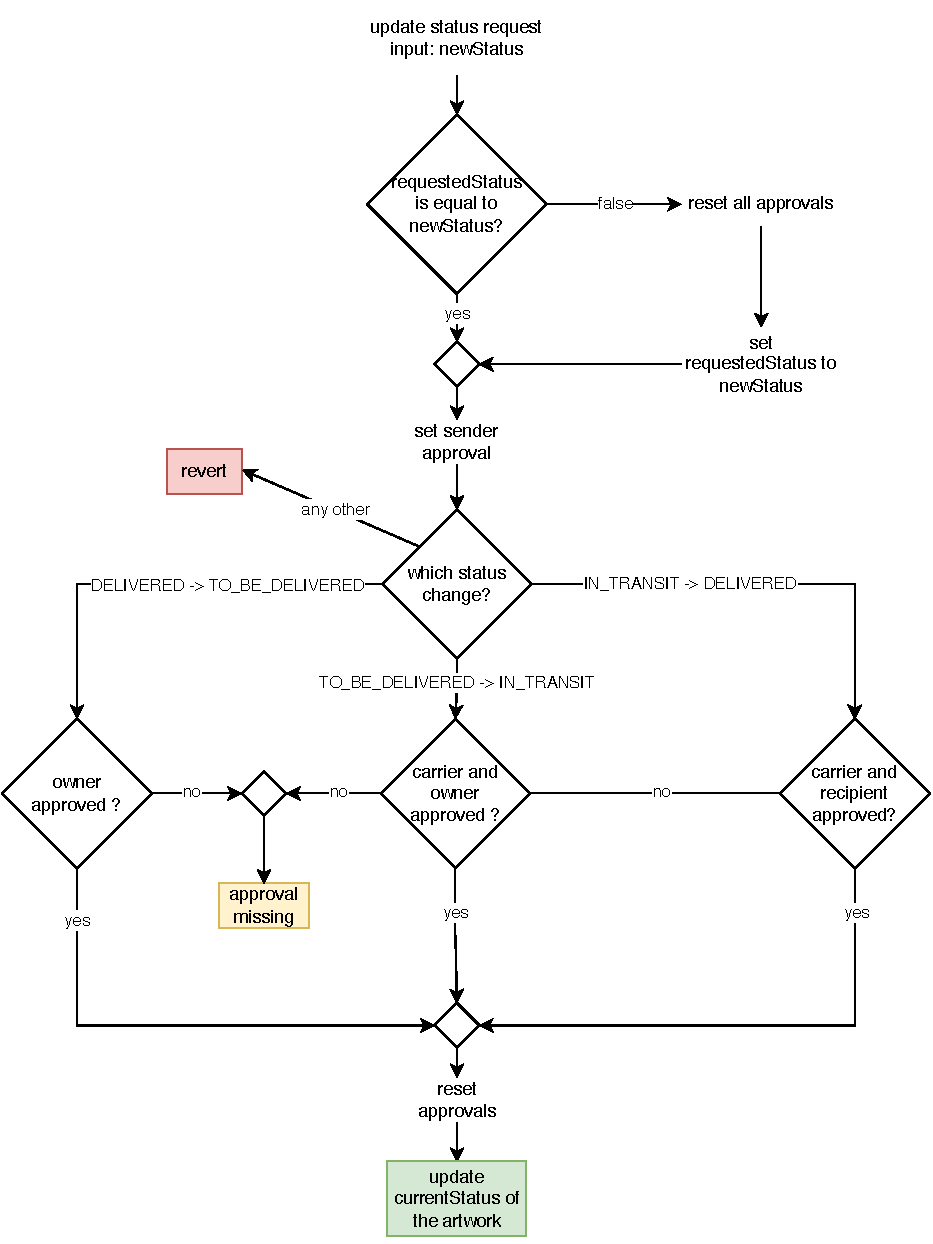
\includegraphics[height=0.5\textheight, keepaspectratio]{diagrams/update_status.drawio.pdf}
    \caption{Multi-approval transportation status change}
    \label{fig:update_status}
\end{figure}

To differentiate between the status that actors want to change to and the status which is currently in place we introduced two variables: \texttt{requestedStatus} and \texttt{currentStatus}. Users are able to request a status change by submitting a new \texttt{requestedStatus}. If this value does not match the previous value all approvals are reset and the \texttt{requestedStatus} field is set to the new value. The next step is to set the approval for the actor who sent the initial update request. Because different actors need to approve for different status changes we need to check for the three distinct cases.

If the status is requested to change from TO\_BE\_DELIVERED to IN\_TRANSIT the carrier and the owner must approve that change. This check is preformed analogously for the change from IN\_TRANSIT to DELIVERED. Lastly the decision to change from DELIVERED to TO\_BE\_DELIVERED is made by the owner alone. Any other combination of status change is not allowed and the transaction will be reverted.

If the right approvals have already been made the function will update the \texttt{currentStatus} automatically and terminate. If any approval is missing it will terminate without updating the \texttt{currentStatus}. In that case the actor in question must submit their own request for a status update.

\subsubsection{getArtworkData}
The function to retrieve data about an artwork is the simplest one. It merely returns the \texttt{ArtworkData} object mapped to the requested artwork id. To easily convert the returned tuple to an object using the contract \gls{abi}, each property is mapped to the tuple entry specified in the function signature, visible in Listing \ref{lst:scget}.

\lstinputlisting[
    language=Solidity,
    caption=\gls{sc} getArtworkData function signature,
    label=lst:scget,
    firstline=150,
    lastline=169
]{codesnippets/smartcontract.sol}


\section{artis-server}


\section{artis-frontend}
